\chapter{Seperating Axis Theorem}

\section{Zasada działania}
Separating Axis Theorem, w skrócie SAT, jest metodą pozwalającą wykryć, czy dane dwa wielokąty wypukłe przecinają się \cite{SAT}. Odpowiednie rozwinięcie algorytmu umożliwia również znalazienie najmniejszego wektora przeniknięcia obiektów.  SAT jest algorytmem genetycznym, który pozwala szybko zweryfikować, czy nastąpiła kolizja między obiektami. Niweluje to konieczność stosowania złożonych obliczeniowo jak i czasowo algorytmów, umożliwiając sprawdzenie kolizji dla duzej liczby obiektów bez spadku wydajności aplikacji.\\
Ogólna zasada działania Separating Axis Theorem polega na sprawdzeniu, czy istnieje oś dzieląca sprawdzane obiekty bez ich przecinania. Jeśli nie jest możliwe znalezienie takiej osi, oznacza to, iż zaistniała kolizja tych obiektów.

\section{Projekcja na płaszczyznę}
Ważnym zagadnieniem podczas omawiania działania algorytmu SAT są projekcje. Ideę projekcji można przedstawić jako cień rzucany przez obiekt na płaszczyznę, gdy światło skierowane jest prostopadle do płaszczyzny a obiekt znajduje się pomiędzy źródłem światła a płaszczyzną.
\begin{figure}[h]
\centering
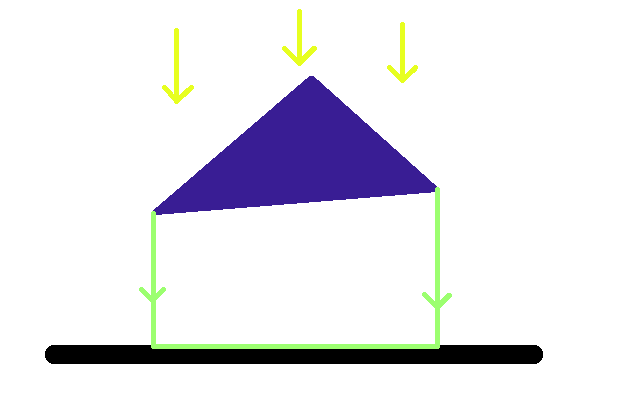
\includegraphics[width=0.4\textwidth]{figures/projection.png}
\caption{Projekcja na płaszczyznę (opracowanie własne).}%
\label{rys:Projekcja na plaszczyzne}
\end{figure}
\newpage
Omówiona w wstępie rozdziału idea algorytmu w praktyce wykorzystuje projekcje i~przedstawia się następująco: jeśli dwa wielokąty wypukłe nie kolidują ze sobą to istnieje co~najmniej jedna oś, dla której projekcje obiektów nie zachodzą na siebie.
\begin{figure}[h]
\centering
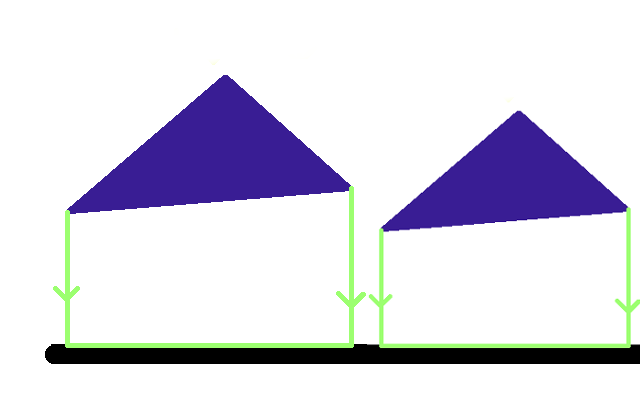
\includegraphics[width=0.5\textwidth]{figures/projection2.png}
\caption{Projekcja na płaszczyznę (opracowanie własne).}%
\label{rys:Projekcja na plaszczyzne}
\end{figure}

\section{Algorytm SAT}
Algorytm wykonuje sprawdzenie nałożenia projekcji obiektów na osie dopóki nie trafi na~pierwszą oś, dla której projekcje nie zachodzą na siebie. Jeśli nie znajdzie takiej osi, zwraca informację o przecinaniu się obiektów. W przeciwnym wypadku dostajemy informacje, że~obiekty nie kolidują. \\
Aby stwierdzić czy projekcje na danej osi się nakładają, należy sprawdzić czy początkowy punkt pierwszego obiektu znajduje się blizej początku osi niż początkowy punkt drugiego sprawdzanego obiektu. Jeśli tak, to następnie wykonujemy sprawdzenie, czy najdalej wysunięty w prawo punkt pierwszego obiektu jest położony dalej niż poczatkowy punkt drugiego obiektu. Jeśli tak jest, oznacza to, iż dla tej osi zachodzi kolizja obiektów. Gdy początek pierwszego obiektu jest położony na osi dalej niż drugi, wykonujemy analogiczne operacje, porównujac najdalej wysunięty punkt drugiej bryły z początkowym punktem projekcji pierwszego. \\
Teoretycznie istnieje nieskończenie wiele osi, które możemy sprawdzić. W praktyce wystarczy sprawdzić jedynie osie wzdłuż normalnych płaszczyzn, z których złożone są sprawdzane bryły oraz wzdłuż osi stworzonych z iloczynów wektorowych brzegów obiektów. Zostało to pokazane na rynunku (5.3). Dla przejrzystego zaprezentowania wszystkich sprawdzanych osi zostały użyte trójkąty.
\begin{figure}[h]
\centering
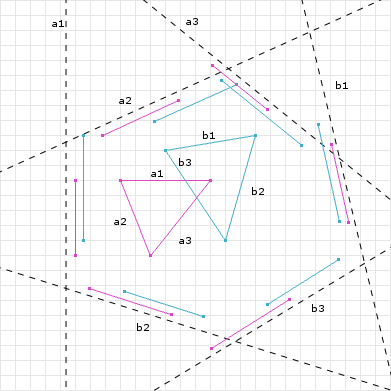
\includegraphics[width=0.5\textwidth]{figures/sat_test.png}
\caption{Sprawdzane osie dla algorytmu SAT\protect\cite{sat_help}.}%
\label{rys:Sprawdzane osie dla algorytmu SAT}
\end{figure}

\section{Iloczyn wektorowy}
Wynikiem iloczynu wektorowego nowy wektor o kierunku prostopadłym do płaszczyzny utworzonej przez mnożone wektory o długości równej iloczynowi długości wektorów oraz sinusa kąta między nimi \cite{math1}. Zwrot utworzonego wektora wyznaczany jest regułą prawej ręki lub regułą śruby prawoskrętnej. Kolejność mnożenia odgrywa tu niemałe znaczenie, ponieważ wynik iloczynu wektorowego AxB nie równa się BxA.
Wartość iloczynu wektorowego zdefiniowana jest następujacym wzorem: \\
\begin{equation}\|\vec{a}\times\vec{b}\|=\|\vec{a}\|\bullet|\vec{b}\|\bullet\sin\gamma\end{equation}
Produkt iloczynu skalarnego wektorów a i b ma postać: \\
\begin{equation}
\centering
a \times b=\vec{a}\times\vec{b}=
=(a\_{x}b\_{z}-a\_{z}b\_{y})\widehat{x}+(a\_{z}b\_{x}-a\_{x}b\_{z})\widehat{y}+(a\_{x}b\_{y}-a\_{y}b\_{y})\widehat{z}
\end{equation}
co równoważne jest z zapisem: \\
\begin{equation}
\centering
\vec{a}\times\vec{b}=[a\_{x}b\_{z}-a\_{z}b\_{y},a\_{z}b\_{x}-a\_{x}b\_{z},a\_{x}b\_{y}-a\_{y}b\_{y}]
\end{equation}
\section{Znalezienie MTV}
MTV (Minimum Translation Vector) jest to wektor opisujący minimalną część wspólną nachodzących obiektów, który jest używany do odepchnięcia kolidująch obiektów do stanu, w którym nie będą już się przecinać \cite{SAT}. W pierwotnej wersji algorytmu SAT otrzymujemy jedynie informację o tym czy kolizja między bryłami zachodzi czy też nie. Jednakże wystarczy zapisywać wielkość nałożenia obiektów podczas sprawdzania ich projekcji i wybrać najmniejsze wartości dla każdej osi, aby otrzymać szukany MTV.

\section{Problemy związane z używaniem Seperating Axis Theorem}
Istnieje kilka zauważalnych wad zastosowania SAT. \\
Pierwszą jest możliwość wykorzystania jedynie brył wypukłych. Jedną metodą na zniwelowanie tej wady jest podzielenie złożonego obiektu na kilka brył tak, aby każda z brył składających się na obiekt była wypukła.\\
Drugą wadą jest sytuacja, w której jeden obiekt jest zawarty w drugim. W takim wypadku obliczony wektor MTV może zawierać błędne wartości oraz zwrot. Rozwiązaniem będzie dodanie do sprawdzania każdej osi testu na zawieranie. \\
Dodatkowo należy pamiętać, że testowane płaszczyzny mogą się powtarzać, np. dla sześcianu wystarczy przestestować trzy płaszczyzny zamiast sześciu, ponieważ dla każdej z równoległych płaszczyzn potrzeba tylko jednego sprawdzenia. Przyspiesza to czas sprawdzania kolizji i znacząco zmniejsza liczbę potrzebnych iteracji.